\chapter{Methodology}
\label{ch:PD}

\section{Environment}

\paragraph{}
Since the time of execution has been focused on in this work, it is important to note the environment in which the tests have been conducted. Table 3.1 shows the system configuration in which the tests have been conducted. Since the focus is on low powered devices, GPU acceleration has not been used in any of the tests.
\begin{table}[h]
    \centering
    \caption{System Specifications}
    \begin{tabular}{| r | l |}
        \hline
        OS & Arch Linux \\
        \hline
        CPU & Intel Core i5-7200U @ 4x 3.1GHz \\
        \hline
        GPU & NVIDIA GeForce 940MX \\
        \hline
        RAM & 8GB \\
        \hline
    \end{tabular}
\end{table}

\paragraph{}
\textbf{Python} language was used to conduct the tests using the interactive environment provided by \textbf{IPython}. The \textbf{scikit-learn} library has been extensively used for training and testing the models. \textbf{Pandas} library has been used along-with \textbf{numpy} to clean and prepare the dataset for processing.

\section{Workflow}
\paragraph{}
To achieve the objectives of the project, the following workflow was planned:
\begin{enumerate}
    \item Find a dataset that meets the present standards
    \item Import, segment and clean the dataset as per requirements
    \item Find important features in the datasets
    \item Decide on performance parameters to use for comparison
    \item Run tests on the dataset with multiple algorithms
    \item Compare the results
\end{enumerate}

\section{Dataset}
\paragraph{}
Two popular datasets were found for the purpose of training and testing IDSs, the KDD'99 \cite{kdd99} and the UNSW-NB15 \cite{unsw15}. KDD'99 presented various problems, such as redundancy, unbalanced sets etc., as discussed thoroughly in \cite{unsw_comparison}. UNSW-NB15, besides being a more recent dataset, hence meeting the present standards in types of data packet and more accurate labels, also addressed issues in the KDD'99 dataset. Hence, the choice of UNSW-NB15 was made for this work.

\section{Cleaning the Dataset}
\paragraph{}
The UNSW-NB15 dataset contains over 2.5 million records, and is split into 4 subsets, each containing 700,000 records. The first subset has been used for training the models, and the second for testing throughout the work. Each subset goes through the following steps before it can be used for building the models:
\begin{enumerate}
    \item Import dataset using python pandas library
    \item Fill empty values (attack\_cat = '' for normal data) with 0
    \item Transform nominal data values to numeric
    \item Add feature names to the pandas dataframe (only for readability while debugging)
\end{enumerate}

\section{Feature Selection}
\label{feature_select}
\paragraph{}
Decision Tree algorithms in scikit-learn library assign an importance score to each feature on the basis of how much they contribute in the classification. The ExtraTreesClassifier class was used to fetch these importance scores (Figure \ref{feature_importance})
\begin{figure}[h]
    \hfill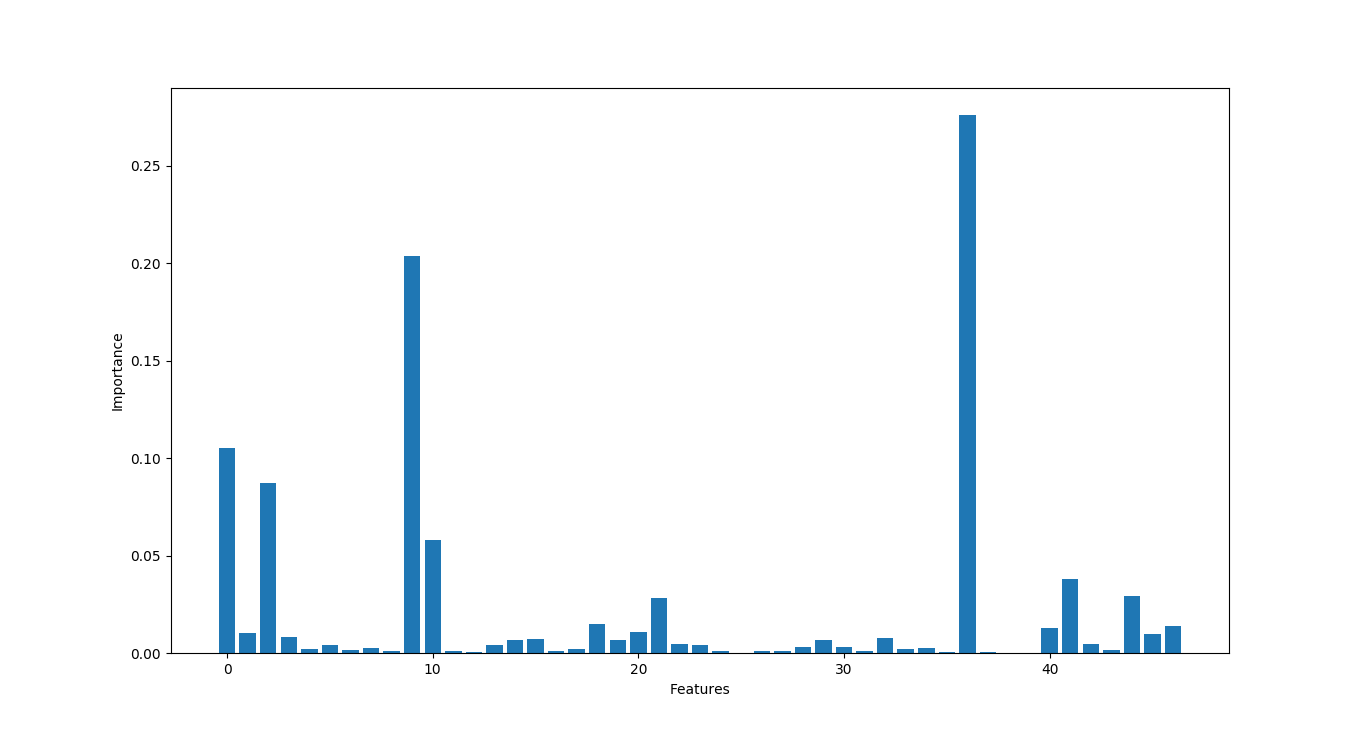
\includegraphics[width=1\textwidth]{Chapter3/feature_importance}\hspace*{\fill}
    \caption{Feature importance}
    \label{feature_importance}
\end{figure}

\paragraph{}
It was observed that 2 features had radically high importance scores (sttl and ct\_state\_ttl). The first one is the source to destination time to live, which makes sense as it is often manipulated to run various kinds of attacks, and the second is an additional generated feature dependent on state, sttl and dttl.

\paragraph{}
The two other peaks in the graph (Figure \ref{feature_importance}), at x = 0 and 2 are source and destination IP addresses. It makes sense that they have a high score as attacks or normal data are likely to originate from the same source and go to the same destination in the dataset curated at a lab at a university, but it is not very useful to build a generic model to classify an attack as it is a property of the source, and not the kind of data packet.

\section{Performance Parameters}
\paragraph{}
A confusion matrix is used to define accuracy of the models. A confusion matrix has 4 parameters:
\begin{itemize}
    \item True Positive (TP): Number of correctly classified attack records
    \item True Negative (TN): Number of correctly classified normal records
    \item False Positive (FP): Number of misclassified attack records
    \item False Negative (FN): Number of misclassified normal records
\end{itemize}
Using these 4 parameters, the accuracy may be calculated as:
\begin{equation}
    accuracy = \frac {TP + TN} {TP + TN + FP + FN}
\end{equation}

\paragraph{}
To factor in the time of execution, two new parameters are introduced. Since the objective is to maximize accuracy and minimize time of execution, the final score of a model is defined as:
\begin{equation}
    score \propto \frac {accuracy} {execution\_time}
\end{equation}
With the proportionality constant as 1, the Training Score (TS) and Prediction Score (PS) are defined as:
\begin{equation}
    TS = \frac {accuracy} {time\_to\_fit/train}
\end{equation}
\begin{equation}
    PS = \frac {accuracy} {time\_to\_predict/classify}
\end{equation}
